\chapter{Pravidla deskové hry}
Hra Logic je desková hra pro dva hráče \cite{Logic_pravidla}. Jeden hráč určí hledanou kombinaci, dále bude označován jako 
hráč~A, a~druhý tuto kombinaci za pomoci logických úvah a~vyhodnocení hráčem~A~hledá, dále bude označován jako hráč~B.

Hráči si určí herní pozice. Hráč~A~vybere barevné kolíky dle libosti a~následně je v~určitém pořadí vloží do zadávacího pole. Zadání zakryje
stříškou, aby tuto
kombinaci spoluhráč neviděl. Hráč~B~se v~tuto chvíli nedívá. Hráč~B~následně zvolí libovolnou kombinaci barev a~jejich pozic. Po 
ukončení tahu nechá
hráče~A,~aby jeho tah vyhodnotil. Hráč~A~vyhodnotí tah následujícím způsobem. Pokud hráč~B~vložil správnou barvu na správnou pozici, tak vloží 
do vyhodnocovací sekce černý kolík. Pokud vložil barvu, která se v~zadání vyskytuje, ale vložil ji na nesprávnou pozici, tak vloží bílý kolík.
Pokud zůstanou některé pozice neobsazené, tak to znamená, že se dané barvy v~zadání nevyskytují. 
Vyhodnocovací kolíky umisťuje od kraje, nejprve černé a~pak bílé, aby hráči~B~nebylo jasné, kterých hracích kolíků se vyhodnocení 
týká \cite{Logic_pravidla}.
Poté začne hráč~B~na základě vyhodnocení a svých všech předchozích tahů hledat správnou kombinaci.

Hráč~B~má maximálně 10~pokusů na zjištění správné kombinace. Po skončení hry hráč~A~odkryje stříšku a~ukáže hledanou kombinaci. Hra skončí po 
určení správné 
kombinace, nebo po vypotřebování všech pokusů.

Hru lze hrát ve více variantách. Hráči se mohou domluvit, zda zadání může, nebo nesmí obsahovat volnou pozici. Zároveň existuje 
více variací této hry. Většinou se liší v~délce hledané kombinace.

\begin{figure}[!h]
  \begin{center}
    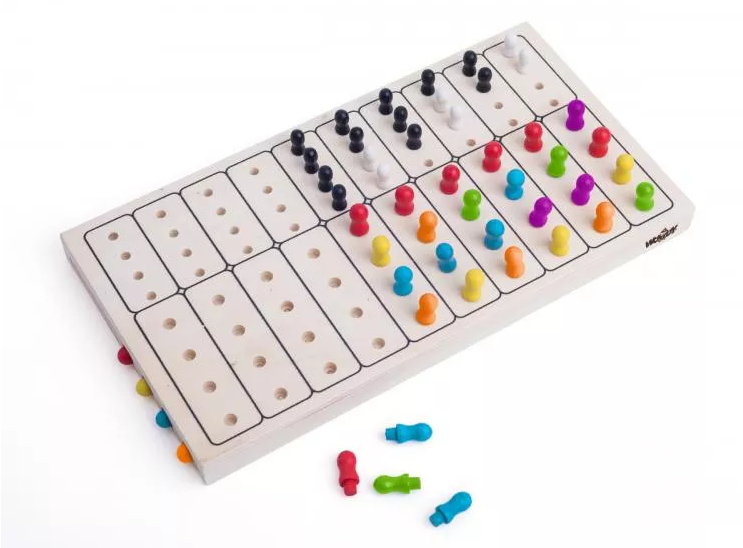
\includegraphics[scale=0.6]{obrazky/Logic_deskovka.png}
  \end{center}
  \caption[Desková hra Logic \cite{Logic_deskovka}]{Desková hra Logic \cite{Logic_deskovka}.}
\end{figure}

\chapter{Návrh elektroniky}
V následující kapitole budou rozebrány všechny komponenty DPS Elektronické hry Logic. Návrh se skládá z řídicí elektroniky, 
napájení, herních prvků a dalších potřebných komponent.

\begin{figure}[!h]
  \begin{center}
    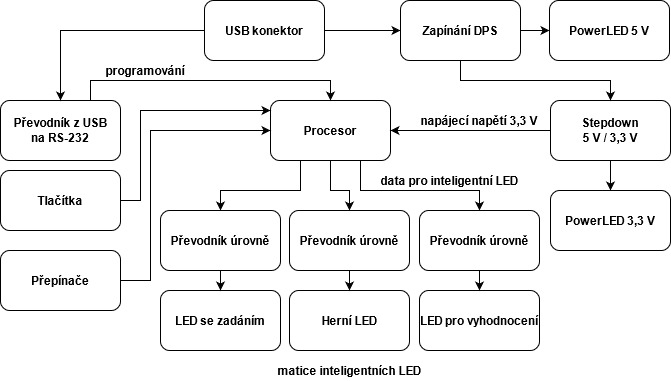
\includegraphics[scale=0.5]{obrazky/v2_blokove_schema.jpg}
  \end{center}
  \caption[Blokové schéma elektroniky]{Blokové schéma elektroniky.}
\end{figure}    

\section{Řídicí elektronika}
Jako řídicí elektronika byl vybrán mikrokontrolér ESP32-PICO-D4. Hlavním důvodem pro výběr tohoto mikrokontroléru bylo, že je téměř totožný 
jako ESP32-WROOM, se 
kterým mám dlouhodobé zkušenosti. Tento mikrokontrolér má veškeré periferie, které jsou pro výrobu této hry zapotřebí. 

Mikrokontrolér ESP32-PICO také podporuje Arduino framework, díky kterému bylo programování značně zjednodušeno.

Mikrokontrolér ESP32-PICO obsahuje \cite{PICO_datasheet}: 
\begin{itemize}
    \item WiFi,
    \item Bluetooth, 
    \item 32~GPIO pinů, 
    \item dvoujádrový 32bitový procesor Xtensa LX6,
    \item 520~kB~SRAM, 
    \item 4~MB~FLASH. 
  \end{itemize}

  Napájecí napětí tohoto mikrokontroléru je od~3,0~do~3,6~V~a průměrný odběr proudu je 80~mA \cite{PICO_datasheet}. ESP32-PICO má vyvedeno 
  32~GPIO pinů, které je 
  možno softwarově nastavit jako vstupní nebo výstupní. Na tyto piny lze poté připojit různá zařízení. Vstupním senzorem může 
  být typicky tlačítko a~výstupním indikátorem např. LED. Tato zařízení zprostředkovávají komunikaci mezi mikrokontrolérem a okolním 
  světem.

  \begin{figure}[!h]
    \begin{center}
      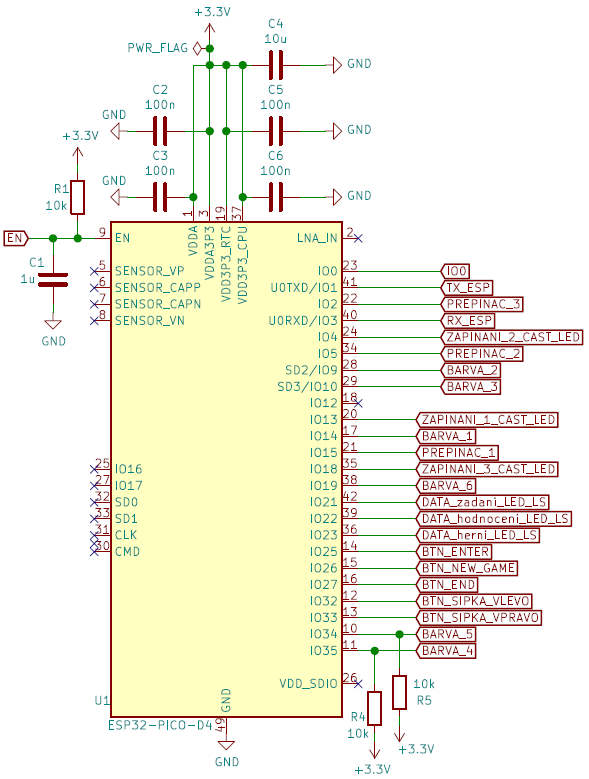
\includegraphics[scale=1]{obrazky/ESP32_PICO_schema.png}
    \end{center}
    \caption[Schéma zapojení mikrokontroléru ESP32-PICO \cite{PICO_datasheet}]{Schéma zapojení mikrokontroléru ESP32-PICO \cite{PICO_datasheet}.}
  \end{figure}

  GPIO piny IO16 a IO17 nemohou být použity, protože ESP32-PICO má na těchto pinech připojenou flash paměť \cite{PICO_datasheet}.
  Pokud by na tento pin bylo připojeno nějaké zařízení, tak by mikrokontrolér ztratil přístup ke své paměti.

  GPIO piny IO02, IO05, IO12 a IO15 slouží jako konfigurační piny při spouštění nebo resetu mikrokontroléru ESP32-PICO. Slouží například k~výběru
  paměti, ze které se mikrokontrolér ESP32-PICO načítá. Při resetu musí být tyto piny ve správné konfiguraci. 

  Pin MTDI je GPIO12 a pin MTDO je pin GPIO15 \cite{PICO_datasheet}.

  \iffalse

  \begin{table}[!h]
    \caption{Konfigurační piny \cite{PICO_datasheet}.}
    \begin{center}
      \begin{tabular}{|c|c|c|c|c|c|}
      \hline
      \rowcolor[HTML]{9B9B9B} 
      \multicolumn{6}{|c|}{\cellcolor[HTML]{9B9B9B}{\color[HTML]{000000} Voltage of Internal LDO (VDD\_SDIO)}} \\ 
      \hline
      \rowcolor[HTML]{C0C0C0} 
      Pin & Default & \multicolumn{2}{c|}{\cellcolor[HTML]{C0C0C0}3.3 V} & \multicolumn{2}{c|}{\cellcolor[HTML]{C0C0C0}1.8 V} \\ 
      \hline
      MTDI & Pull-down  & \multicolumn{2}{c|}{0}   & \multicolumn{2}{c|}{1}  \\ 
      \hline
      \rowcolor[HTML]{9B9B9B} 
      \multicolumn{6}{|c|}{\cellcolor[HTML]{9B9B9B}{\color[HTML]{000000} Booting Mode}}  \\ 
      \hline
      \rowcolor[HTML]{C0C0C0} 
      Pin  & Default & \multicolumn{2}{c|}{\cellcolor[HTML]{C0C0C0}SPI Boot}   & \multicolumn{2}{c|}{\cellcolor[HTML]{C0C0C0}Download Boot} \\ 
      \hline
      GPIO0  & Pull-up  & \multicolumn{2}{c|}{1} & \multicolumn{2}{c|}{0} \\ 
      \hline
      GPIO2  & Pull-down & \multicolumn{2}{c|}{Don't-care}  & \multicolumn{2}{c|}{0}  \\ 
      \hline
      \rowcolor[HTML]{9B9B9B} 
      \multicolumn{6}{|c|}{\cellcolor[HTML]{9B9B9B}Enabling/Disabling Debugging Log Print over U0TXD During Booting} \\ 
      \hline
      \rowcolor[HTML]{C0C0C0} 
      Pin  & Default  & \multicolumn{2}{c|}{\cellcolor[HTML]{C0C0C0}U0TXD Active} & \multicolumn{2}{c|}{\cellcolor[HTML]{C0C0C0}U0TXD Silent} \\ 
      \hline
      MTDO & Pull-up & \multicolumn{2}{c|}{1}  & \multicolumn{2}{c|}{0} \\ 
      \hline
      \rowcolor[HTML]{9B9B9B} 
      \multicolumn{6}{|c|}{\cellcolor[HTML]{9B9B9B}Timing of SDIO Slave} \\ 
      \hline
      \rowcolor[HTML]{C0C0C0} 
      {\color[HTML]{000000} Pin} & {\color[HTML]{000000} Default} & {\color[HTML]{000000} \begin{tabular}[c]{@{}c@{}}FE Sampling\\ FE Output\end{tabular}} & {\color[HTML]{000000} \begin{tabular}[c]{@{}c@{}}FE Sampling\\ RE Output\end{tabular}} & {\color[HTML]{000000} \begin{tabular}[c]{@{}c@{}}RE Sampling\\ FE Output\end{tabular}} & {\color[HTML]{000000} \begin{tabular}[c]{@{}c@{}}RE Sampling\\ RE Output\end{tabular}} \\ 
      \hline
      MTDO  & Pull-up  & 0    & 0   & 1  & 1 \\ 
      \hline
      GPIO5  & Pull-up  & 0  & 1 & 0  & 1 \\ 
      \hline
      \end{tabular}  
    \end{center}
  \end{table}

\fi

  GPIO piny IO34 a~vyšší jsou pouze vstupní \cite{PICO_datasheet}. Vstupní piny nemají softwarově zapojitelný pullup rezistor. 
  Pokud je tedy zapotřebí pullup rezistor, musí se fyzicky zapojit.
  
  \section{Napájení}
  Napájení probíhá před USB konektor. V dnešní době jsou 2 nejpoužívanější konektory – USB Micro a USB-C. Proto byly navrženy oba USB konektory. 
  DPS nepodporuje funkci Quick Charge ani Power Delivery. DPS může být napájena pouze napětím 5 V. Každé jiné napětí by zbytečné komplikovalo návrh DPS.
  Konektor USB-C je tedy funkčně zapojen totožně jako USB Micro a oba konektory jsou na DPS pouze kvůli jejich tvaru. 
  
  \begin{figure}[!h]
    \begin{center}
      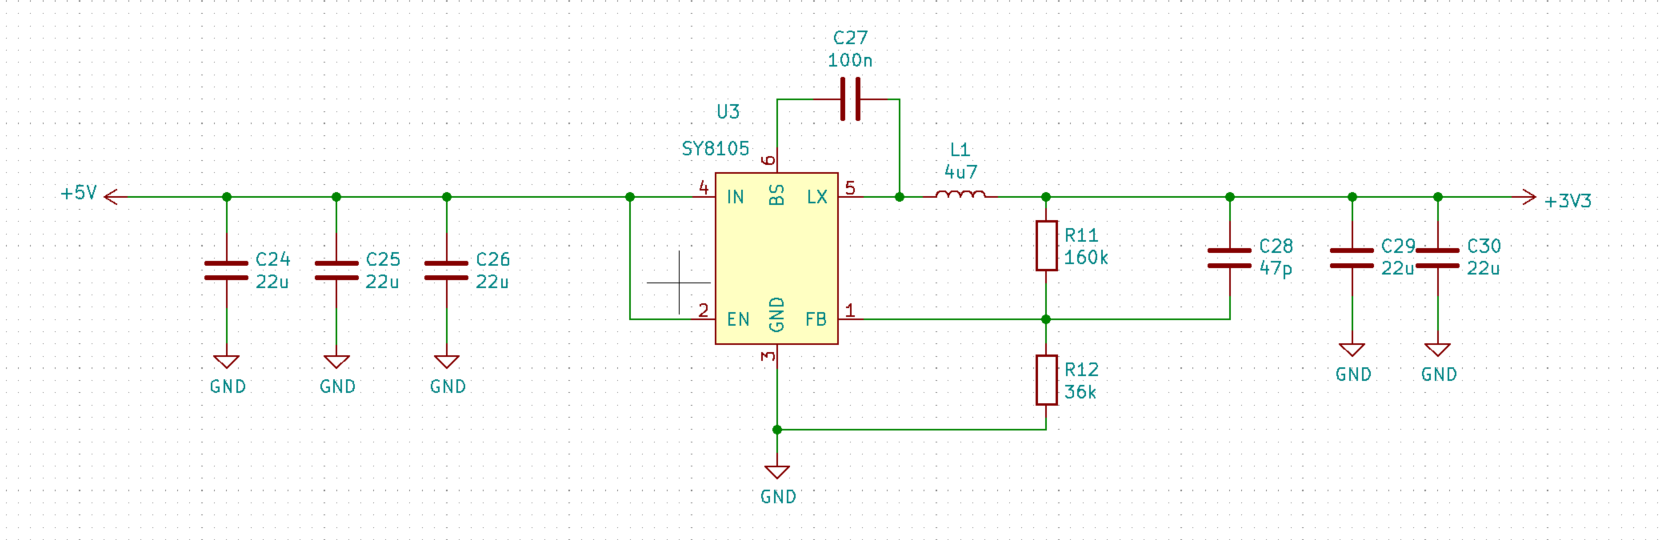
\includegraphics[scale=0.4]{obrazky/SY8105_schema.png} %vyměnit za správný obrázek
    \end{center}
    \caption[Schéma zapojení konektoru USB-C \cite{USB-C}]{Schéma zapojení konektoru USB-C \cite{USB-C}.}
  \end{figure}

  \section{Snižující měnič napájecího napětí pro mikrokontrolér}
  Mikrokontrolér ESP32-PICO má napájecí napětí 3,3~V. Napětí z~powerbanky přes USB je 5~V. Proto je tedy zapotřebí zapojit 
  měnič pro snížení napětí, který bude vytvářet z~napájecího napětí 5~V napájecí napětí 3,3~V pro mikrokontrolér ESP32-PICO.

  Jako měnič byl zvolen čip SY8105. Tento čip byl vybrán podle projektu RB0005-UniversalStepDown \cite{UniversalStepDown}. 
  V~tomto projektu zapojení funguje bezproblémově, a~proto bylo rozhodnuto toto zapojení použít v~mé práci. 

  \begin{figure}[!h]
    \begin{center}
      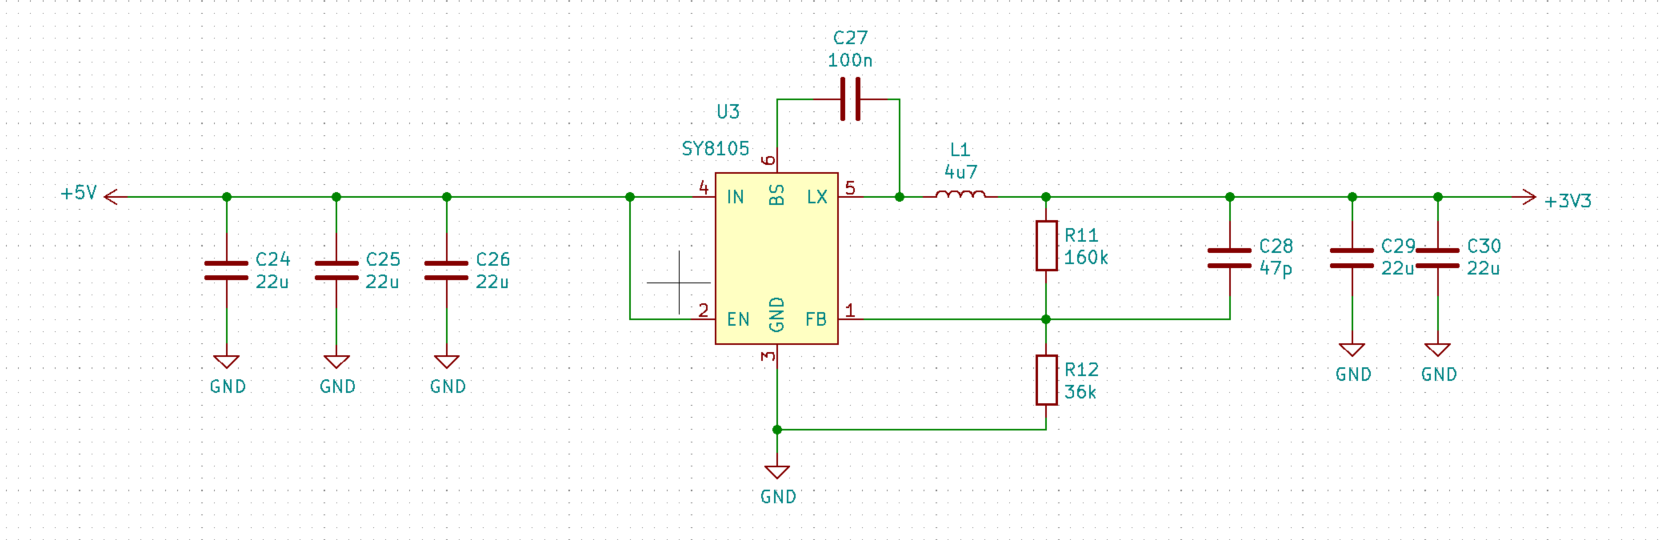
\includegraphics[scale=0.4]{obrazky/SY8105_schema.png}
    \end{center}
    \caption[Schéma zapojení čipu SY8105 \cite{SY8105_datasheet}]{Schéma zapojení čipu SY8105 \cite{SY8105_datasheet}.}
  \end{figure}

  Výstupní napětí zapojení čipu SY8105 je závislé na poměru rezistorů R11~a~R12 \cite{SY8105_datasheet}. 
  Hodnota rezistoru R11 byla zvolena 160 k$\Omega$. Hodnota rezistoru R12 byla dopočítána dle následující rovnice. %odkaz na rovnici (dle rovnice číslo...)

  \begin{equation} 
    R_{12}~=~\frac{0,6}{U_{OUT}-0,6}~\cdot~R_{11}~=~\frac{0,6}{3,3-0,6}~\cdot~160\cdot10^3~=~35,555~\:k\Omega 
    \quad \quad \quad \cite{SY8105_datasheet}
  \end{equation}

  Hodnota rezistoru R12 byla zvolena nejbližší z vyráběné rezistorové řady E24 \cite{Rezistorova_rada}, tudíž 36 k$\Omega$. Hodnota 
  rezistoru se musí co nejvíce blížit vypočítané hodnotě, aby výstupní napětí nebylo příliš odlišné od požadovaného. Proto nebyl
  zvolen rezistor z častěji používaných řad E6 ani E12. Hodnota rezistoru z těchto řad by se již příliš odchylovala od vypočítané.
   
  %popsat funkci zapojení

  \begin{table}[!h]
    \caption{Parametry čipu SY8105 \cite{SY8105_datasheet}}
    \begin{center}
        \begin{tabular}{|c|c|}
            \hline
            Vstupní napětí             & 4,5--18~V \\ 
            \hline
            Maximální výstupní proud   & 5~A \\
            \hline
        \end{tabular}    
    \end{center}
\end{table}

  \section{Převodník z~USB na RS-232}
  Mikrokontrolér ESP32-PICO používá jako komunikační rozhraní linku RS-232. Programování ale probíhá přes USB konektor, který toto rozhraní
  nemá. Proto bylo potřeba použít převodník z~USB na rozhraní RS-232.
  
  Velkou inspirací při výběru součástek byl kit ESP32-DEVKITC \cite{Devkit_schema}. Tento kit obsahuje ESP32-WROOM a~také převodník
  z~USB na RS-232. Na tomto kitu je převodník realizován čipem CP2102. ESP32-WROOM a~ESP32-PICO se liší pouze v~drobnostech. 
  Proto byl převodník CP2102 použit i~při návrhu převodníku u~elektronické hry Logic.  Tento čip zároveň převádí logiku 
  z~0--5~V~na logiku 0--3,3~V \cite{CP2102_datasheet}. 

  \begin{table}[!h]
    \caption{Parametry čipu CP2102 \cite{CP2102_datasheet}}
    \begin{center}
        \begin{tabular}{|c|c|}
            \hline
            Typický odběr proudu   & 9,5~mA \\ 
            \hline
            Napájecí napětí        & 3--3,6 V \\
            \hline
        \end{tabular}    
    \end{center}
  \end{table}

  Čip CP2102 dokáže komunikovat velkým množstvím komunikačních rychlostí (300, 9600, 19200, 38400, 115200, 256000~Bd, atd) 
  \cite{CP2102_datasheet}. Počítač započne komunikaci určitou rychlostí a~tento čip komunikaci zachytí, určí rychlost 
  a~touto rychlostí začne probíhat programování.

  \begin{figure}[!h]
      \begin{center}
        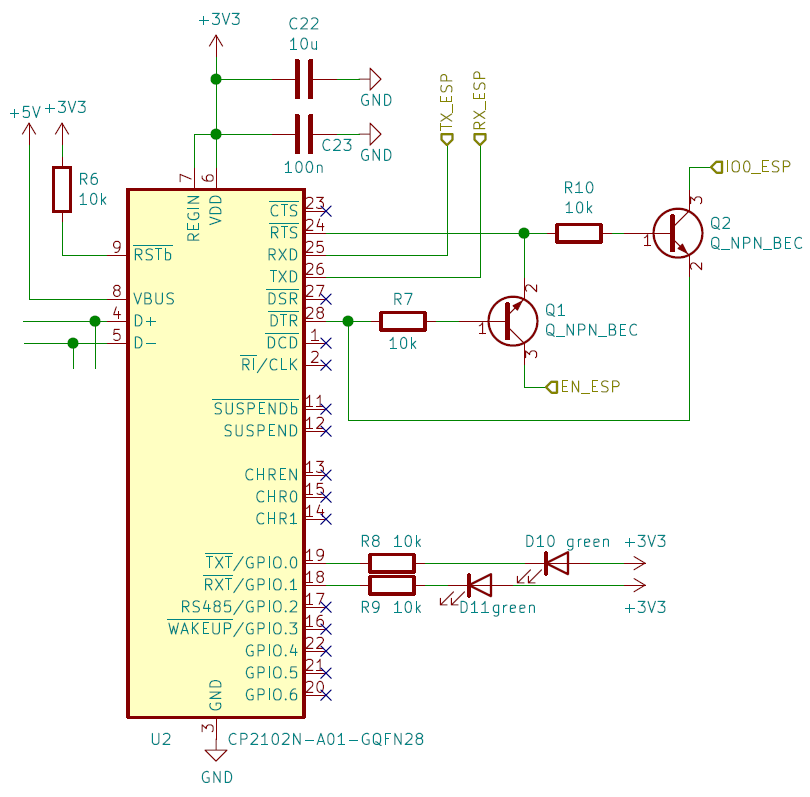
\includegraphics[scale=0.6]{obrazky/CP2102_schema.png}
      \end{center}
      \caption[Schéma zapojení převodníku z~USB na RS-232 \cite{Devkit_schema}]{Schéma zapojení převodníku z~USB na RS-232 \cite{Devkit_schema}.}
  \end{figure}

  Z~USB jsou signály D+~a~D- připojeny k~čipu CP2102. Tento čip signál z~USB převede na signály RX~a~TX, které mají výstup 
  na pinech RXD~a~TXD. Následně jsou tyto signály připojeny k~mikrokontroléru ESP32-PICO. Signály RX~a~TX musí být překříženy~–~RX 
  CP2102 je připojeno na TX ESP32-PICO a~TX CP2102 je připojeno na RX ESP32-PICO. 

  LED~D10~a~D11 slouží k~indikaci komunikace s~mikrokontrolérem ESP32-PICO. Pokud je do mikrokontroléru nahráván program, tak LED~D10~a~D11 
  blikají.

  \begin{figure}[!h]
      \begin{center}
        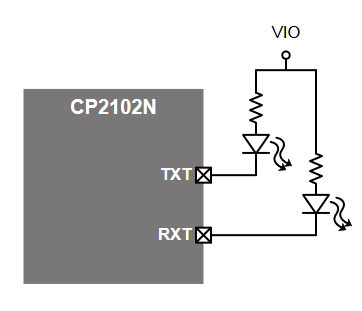
\includegraphics[scale=0.5]{obrazky/CP2102_LED.png}
      \end{center}
      \caption[Zapojení LED pro indikaci komunikace čipu CP2102 s~mikrokontrolérem \cite{CP2102_datasheet}]{Zapojení LED pro indikaci 
      komunikace čipu CP2102 s~mikrokontrolérem \cite{CP2102_datasheet}.}
  \end{figure}

  \section{Herní prvky}
  Herními prvky elektronické hry Logic jsou inteligentní LED typu WS2812C. Tento typ inteligentních LED je určen pro přenosná 
  zařízení díky jejich nízké spotřebě. Jsou také plně kompatibilní s~typem WS2812B \cite{WS2812C_datasheet}. K~těmto inteligentním LED 
  existují knihovny, které usnadňují softwarovou práci s~nimi.

  \begin{figure}[!h]
    \begin{center}
      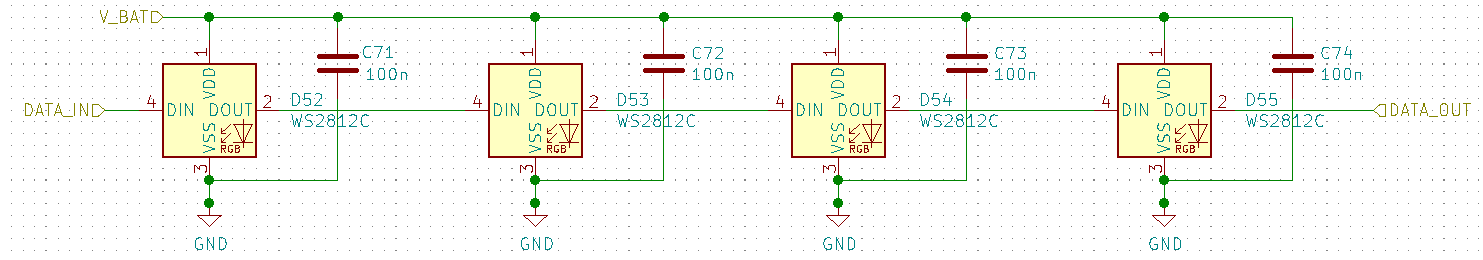
\includegraphics[scale=0.5]{obrazky/WS2812C_spojeni.png}
    \end{center}
    \caption[Zapojení inteligentních LED WS2812C \cite{WS2812C_datasheet}]{Zapojení inteligentních LED WS2812C \cite{WS2812C_datasheet}.}
  \end{figure}

  Každá inteligentní LED má v~sobě procesor, který slouží pro zpracování dat. 
  Inteligentní LED WS2812C se zapojují za sebou přes piny DATA~IN a~DATA~OUT. Každá inteligentní LED převezme data z~pinu 
  DATA~IN, která jsou pro ni určena, a~zbytek pošle ven přes pin DATA~OUT. K pinu DATA~OUT je připojen pin DATA~IN další inteligentí LED. 

  \begin{table}[!h]
    \caption{Parametry inteligentních LED WS2812C \cite{WS2812C_datasheet}}
    \begin{center}
        \begin{tabular}{|c|c|}
            \hline
            Napájecí napětí       & 3,5--5,3~V \\
            \hline
            Výstupní napětí       & (VDD~-~0,5)--(VDD~+~0,5)~V \\
            \hline
            Typický odběr proudu  & 5~mA \\
            \hline
            Klidový odběr proudu  & 0,3~mA \\
            \hline
        \end{tabular}    
    \end{center}
  \end{table}

  Ke každé inteligentní LED je připojen na napájení filtrační kondenzátor \cite{WS2812C_datasheet}, aby LED svítily kontinuálně 
  a~nedostal se jim na napájení žádný šum.

  \subsection{Rozdělení}
  Inteligentní LED jsou rozděneny do tří skupin. Skupina inteligentních LED pro zadání, skupina inteligentních LED pro herní pole 
  a~skupina inteligentních LED pro zobrazení vyhodnocení tahu.
  Skupina inteligentních LED pro zadání obsahuje 4~LED a~skupiny pro herní pole a~pro vyhodnocení každá 40~LED.

  \subsection{Převodník úrovně}
  Inteligentní LED WS2812C pracují s logikou od 0~V do 5~V. Mikrokontrolér ESP32-PICO pracuje s logikou od 0~V do 3,3~V. 
  Z tohoto důvodu byl mezi mikrokontrolér a inteligentní LED na datový signál pro inteligentní LED zapojen převodník úrovně, 
  tzv. level shifter. 
  
  Převodník je realizován MOSFET tranzistorem a dvěma pull-up rezistory. Jeden rezistor je připojen k napájecímu napětí 3,3 V a druhý k 
  napájecímu napětí 5 V. Jedná se o nejjednodušší způsob převodníku úrovně směrem nahoru. Tento způsob umožňuje komunikaci oběma směry. 
  MOSFET tranzistor byl zvolen pro nulovou spotřebu, narozdíl od bipolárních tranzistorů. 

  %Obrázek zapojení level shifteru

  Pokud jsou obě zařízení v klidu (nekomunikují), tak je tranzistor zavřený a pull-up rezistory zajišťují, že na pinu mikrokoltroléru
  i inteligentní LED je logická 1. Pro mikrokontrolér ESP32-PICO je to tedy 3,3 V a pro inteligentní LED WS2812C je to 5 V. Jakmile započne
  mikrokontrolér komunikaci, to znamená, že svůj stav přepne do stavu logické nuly (0 V), tak rozdíl mezi gate a source tranzistoru stoupne
  a na výstupu tranzistoru bude také logická nula (0 V). Pokud by komunikace mohla probíhat i naopak (inteligentní LED by odesílala data do
  mikrokoltroléru), tak by byl princip totožný. 

  \subsection{Zapínání napájení}
  DPS je navrhována pro přenosnou aplikaci, a~proto je potřeba zajistit její co nejnižší odběr. 

  Inteligentní LED WS2812C mají spotřebu 0,3~mA ve vypnutém stavu. Proto je herní pole dohromady
  s~vyhodnocovacími LED rozděleno na 3~části.Tyto 3 části mají rozděleno napájení, které je postupně zapínáno dle potřeby. 
  Do první části patří inteligentní LED se zadáním a~první 4~čtveřice inteligentních LED 
  z~herního pole a~z~vyhodnocení. Do druhé části patří další 3~čtveřice inteligentních LED z~herního a vyhodnocovacího pole. 
  Do třetí části patří poslední 3 čtveřice inteligentních LED z~herního a z vyhodnocovacího pole.

  Ke spínání slouží obvody s~MOSFET tranzistory. MOSFET tranzistory byly zvoleny pro jejich nulovou spotřebu, narozdíl od 
  bipolárních tranzistorů. 

  \begin{figure}[!h]
    \begin{center}
      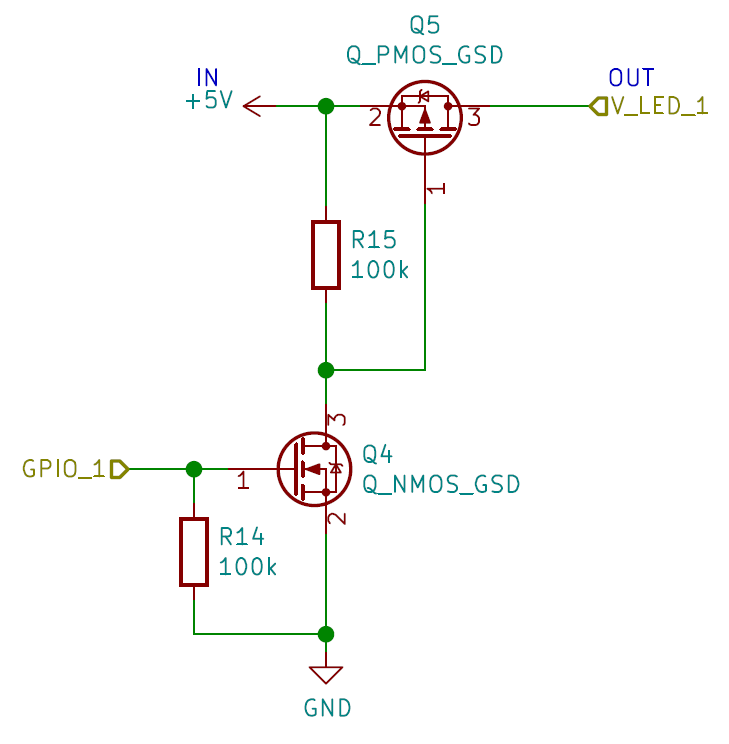
\includegraphics[scale=0.7]{obrazky/Zapinani_napajeni_LED.png}
    \end{center}
    \caption[Obvod pro zapínání napájení pro inteligentní LED]{Obvod pro zapínání napájení pro inteligentní LED.}
  \end{figure}

  Napájení inteligentních LED nelze spínat pouze jedním tranzistorem, protože logická~1~mikrokontroléru ESP32-PICO má hodnotu pouze 3,3~V. 
  V tomto případě je zapotřebí spínat 5~V. Pokud by byl pro spínání použit pouze jeden tranzistor, tak by bylo napájení vždy sepnuto.

  GPIO pin mikrokontroléru ESP32-PICO je nastaven do logické~0, dokud není potřebné přivedení napájecího napětí dané skupině. 
  Při logické nule na gate 
  tranzistoru Q4 je tranzistor zavřený. Tranzistor Q5 v~tomto okamžiku drží zavřený rezistor R15.

  Když je GPIO pin mikrokontroléru přepnut do logické~1, tak se tranzistor Q4 otevře. Otevřením tranzistoru Q4 je gate tranzistoru Q5 
  připojen ke GND a~tím se otevře i~tranzistor Q5, kterým je sepnuto napájecí napětí dané skupině inteligentních LED.

  Rezistor R14 udržuje tranzistor Q4 zavřený při nestandardních stavech pinu mikrokontroléru, jako je např. při resetu procesoru.

  \section{Spínací prvky}
  Přepínač SW1 slouží pro zapínání celé DPS. Tento přepínač připojuje napájecí napětí 5~V~z~USB k~celému zbytku DPS. 
  %doplnit info o kolébkovém vypínači - možná až do realizace

  Tlačítka slouží pro ovládání hry. Ke každému tlačítku je připojen kondenzátor o~hodnotě 100~nF. Tento kondenzátor 
  slouží pro filtraci zákmitů při zmáčknutí tlačítka. Filtrace se proto nemusí řešit softwarově.

  \begin{figure}[!h]
    \begin{center}
      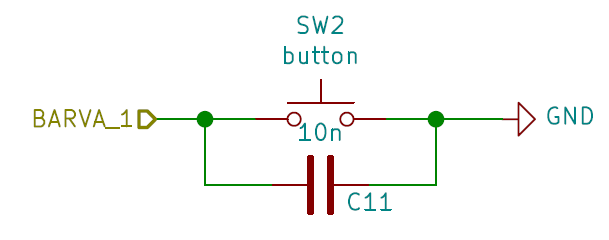
\includegraphics[scale=0.8]{obrazky/Tlacitka_zapojeni.png}
    \end{center}
    \caption[Zapojení tlačítek]{Zapojení tlačítek.}
  \end{figure}

  Přepínače slouží pro volbu možnosti hry. První přepínač slouží pro volbu hry pro jednoho, nebo pro 2 hráče. Druhý 
  slouží pro možnosti hry na 3 nebo 4 herní prvky a poslední přepínač slouží pro nastavení, zda se v zadání může, nebo 
  nesmí vyskytnout mezera. 
  
  Z důvodu nedostatku pinů musely být přepínače připojeny k mikrokontroléru ESP32 přes konfigurační piny. U konfiguračních pinů
  musejí být dodržena pravidla pro připojovaná zařízení.  %(viz kapitola Řídicí elektronika) 
  Z těchto důvodů je jeden přepínač připojen přes pull-down rezistor a ostatní dva přepínače jsou připojeny přes pull-up rezistor. 
  %obrázek připojení přepínačů (možná)

  \begin{table}[!h]
    \caption{Zapojení přepínačů ke strapping pins mikrokontroléru EPS32}
    \begin{center}
        \begin{tabular}{|c|c|c|c|}
            \hline
            {\bf Přepínač}   & {\bf Pin mikrokontroléru} & {\bf Typ připojení rezistoru} \\
            \hline
            SW14      & GPIO15 & Pull-up \\
            \hline
            SW13      & GPIO05 & Pull-up \\
            \hline
            SW15      & GPIO02 & Pull-down \\
            \hline
        \end{tabular}    
    \end{center}
  \end{table}

  \section{Indikace přítomnosti napájecího napětí}
  Pro indikaci přítomnosti napájecího napětí slouží LED~D1~a~D2. LED~D1 indikuje přítomnost napájecího napětí 
  5~V~a~LED~D2 indikuje přítomnost napájecího napětí 3,3~V. Obě LED mají zelenou barvu a jsou připojeny přes
  rezistor o hodnotě 10 k$\Omega$.

  \begin{figure}[!h]
    \begin{center}
      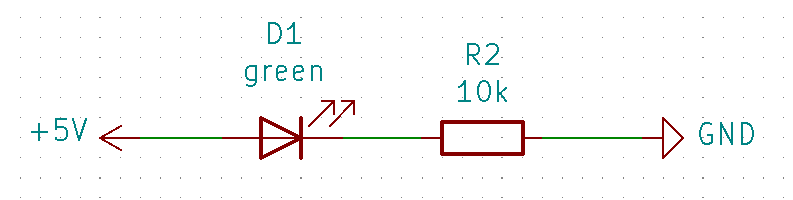
\includegraphics[scale=0.5]{obrazky/powerLED.png}
    \end{center}
    \caption[Zapojení LED pro indikaci napájecího napětí]{Zapojení LED pro indikaci napájecího napětí.}
  \end{figure}

  \chapter{Návrh DPS}
  DPS je navržena v~programu KiCad a~její parametry jsou určeny pro výrobu i~osazení ve firmě JLCPCB \cite{KiCad} \cite{JLCPCB}. Výrobní 
  podklady proto musely být navrženy v~souladu s~jejich výrobními možnostmi \cite{JLCPCB_Capabilities}.

  DPS má 4~vrstvy. Vnitřní vrstvy slouží pro napájení a~vnější pro signálové dráhy. V~jedné vnitřní vrstvě je po celé její ploše 
  polygon GND a~ve druhé vnitřní vrstvě jsou polygony jednotlivých napájecích napětí. Součástky jsou rozloženy tak, aby pokud možno
  korespondovaly s polygony a napájecí napětí tak nemuselo být dále rozváděno zbytečně po celé DPS. Někdy však nemohlo být umístění 
  přizpůsobeno a napájecí napětí tak muselo být přivedenou dráhou v horní nebo spodní vstvě, která jsou převážně určeny pro signálové 
  dráhy. 

  Na vrchní straně jsou umístěny plošky pro osazení součástek, protože firma JLCPCB osazuje součástky pouze z~jedné strany DPS.

  Signálové dráhy jsou vedeny tenkou dráhou a~napájecí dráhy jsou vedeny širší dráhou. V~signálových drahách tečou zanedbatelné 
  proudy, proto mohou být co nejtenčí. Výrobce umožňuje vyrobit u~čtyřvrstvé DPS nejtenčí dráhu 0,09~mm \cite{JLCPCB_Capabilities}. 
  Aby nebyly použity krajní hodnoty, byla zvolena šířka signálové dráhy 0,15~mm.

  Dráhy, kterými je vedeno napájecí napětí, mají tloušťku 0,5~mm. Pro výpočet šířky dráhy byla použita online kalkulačka Printed
  Circuit Board Width Tool \cite{Kalkulacka_drahy_DPS}. Proud dráhami při použití všech inteligentních LED je 420~mA a tloušťka 
  mědi 35~$\mu$A \cite{JLCPCB_Capabilities}. Doporučená šířka dráhy byla tedy 0,236~mm, a~proto byla zvolena šířka dráhy 0,5~mm.

  n~=~84~ks

  $I_\textind{LED}$~=~5~mA 

  \begin{equation} 
    I~=~I_{LED}~\cdot~n~=~5~\cdot~84~=~420~\:~mA
  \end{equation}

  Vnější vrstvy byly vyplněny polygonem GND. Zejména tak bylo učiněno kvůli výrobnímu procesu nanášení nepájivé masky. Tato maska
  může být velmi tenká zejména na plochách, kde jsou pouze tenké dráhy a žádné velké plochy. Vytvořením polygonu GND tak dopomáhá k 
  vytvoření pevné a stejně tlusté nepájivé masky. 

  \section{Vzhled DPS}
  Vzhled DPS byl ovlivněn vzhledem deskové hry a~výrobními možnostmi firmy JLCPCB. Firma JLCPCB vyrábí DPS o~maximálních %není pravda - opravit - asi napsat osazuje/bez velkého poplatku
  rozměrech 10~$\times$~10~cm \cite{JLCPCB}. Tato DPS tedy byla navržena na maximální vyrobitelnou velikost a~poté byly do těchto 
  rozměrů rozmisťovány součástky.

  Inteligentní LED WS2812C jsou rozděleny do 3~skupin, aby se hra co nejvíce podobala deskové hře. Zároveň dopomáhá orientaci ve hře.
  Také kvůli množství inteligentních LED a~jejich poměrně velkým rozměrům (5~$\times$~5~mm) zabírají velkou část DPS 
  \cite{WS2812C_datasheet}. Proto musely být inteligentní LED rozmístěny jako první.

  Inteligentní LED pro zadání jsou umístěny v~horní části DPS. V~levém sloupci pod zadáním se nachází matice inteligentních LED, které slouží jako herní 
  pole, a~v~pravém sloupci je matice inteligentní LED pro vyhodnocení tahu. Matice reprezentují herní tahy, proto jsou v rozložení (4~$\times$~10~LED).
  
  Rozmístění tlačítek a přepínačů probíhalo dle 
  rozmyšlenému způsobu ovládání elektronické hry. Byl také brán ohled na estetiku vzhledu. Proto byly tlačítka i inteligentní LED
  rozmístěny dle přesné mřížky. Následně byl ostatními obvody využíván zbylý prostor. 

  Dráhy s~napájecím napětím by měly být co nejkratší a měly by být vedeny co nejvíce zpříma. Proto byla snaha o umístění součástkek
  se stejným napájecím napětím k sobě. Ne vždy ale mohla být tato doporučení splněna. Někdy musel být proveden kompromis mezi vzhledem a funkčním 
  zapoením. 
  Dílčí obvody byly rozmístěny v~následujícím pořadí~-~USB konektory, měnič napětí, převodník z~USB 
  na RS-232 a~ESP332-PICO. USB konektor musel být umístěn na okraj DPS. Proto byly jednotlivé části obvodu naskládány podél levého okraje DPS.

  USB konektory jsou umístěny těsně vedle sebe. Tímto způsobem je ošetřeno, že za pomoci běžného USB kabelu, nepůjde zapojit napájení do obou 
  konektorů zároveň. 

  Převodník úrovně je umístěn vždy těsně před vstupem signálu do první inteligentní LED daného řetězce.

  Přepínač pro změnu hry pro jednoho a pro 2 hráče byl umístěn do mezery, mezi herní a vyhodnocovací inteligentní LED. Další 2 přepínače, jeden 
  pro volbu hry na 3 nebo 4 herní prvky a druhý na volbu nastavení, zda se v zadání může, nebo nesmí vyskytnout mezera, jsou umístěny v pravém 
  horním rohu. 

  Obvody pro zapínání napájení jednotlivým sekcím inteligentních LED jsou umístěny vždy na začátku dané části polygonu vlevo od herních inteligentních
  LED.
  %(co ještě chybí?)

  \section{Funkční rozmístění součástek}
  U~některých součástek není jejich umístění na DPS lhostejné. Rozmístění součástekv některých případech může ovlivnit funkčnost obvodu. 
  Rozmístění součástek často souvisí s~rozkreslením ve schématu. Například kondenzátory filtrující napájení se umisťují co nejblíže přívodu napájení.

  Rozložení součástek měniče napětí na DPS může velmi ovlivnit jeho funkčnost, zejména pak jeho účinnost. Proto bylo rozložení a~zapojení součástek 
  převzato z~datasheetu.

  \begin{figure}[!h]
    \begin{center}
      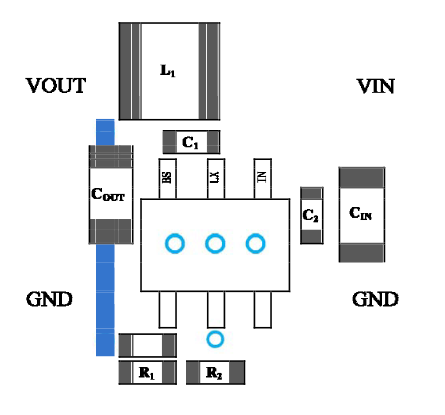
\includegraphics[scale=1]{obrazky/SY8105_rozlozeni_na_DPS.png}
    \end{center}
    \caption[Rozložení součástek kolem čipu SY8105 na DPS \cite{SY8105_datasheet}]{Rozložení součástek kolem čipu SY8105 na DPS 
    \cite{SY8105_datasheet}.}
  \end{figure}

  Signály D+~a~D- od USB k~čipu CP2102 jsou diferenciální pár, a~proto tomu musely být přizpůsobeny i~dráhy těchto signálů. Dráhy 
  jsou vedeny vedle sebe a~blízko u~sebe po celou jejich délku.

  Kondenzátory u~mikrokontroléru ESP32-PICO a~u~čipu CP2102 musí být umístěny co nejblíže jejich pouzdru. Tyto kondenzátory slouží pro 
  filtraci šumu na napájení. Stejná pravidla platí také pro filtrační kondenzátory u inteligentních LED WS2812C.

  Kondenzátory u~tlačítek jsou také umístěny co nejblíže pouzdru tlačítek. Čím blíže pouzdru kondenzátor bude, tím lépe budou 
  filtrovány zákmity při stisku tlačítka.

  \chapter{Oživení DPS}
  Při výrobě finální verze DPS elektronické hry Logic byly využity maximální možnosti osazení firmou JLCPCB.  
  Pro oživení finální DPS je tedy zapotřebí pájení pouze vypínače, který není umístěn na DPS, ale je zasazen do krabičky a zapájen
  do DPS pomocí drátových prodlužek. 

  Při objednání finální DPS nastaly problémy s nedostatkem součástek, se kterým se v této době potýká mnoho návrhářů. Čip SY8105 neměla %citace o nedostatku součástek
  firma JLCPCB dlouhodobě na skladě a nebylo možné čekat, než jej znovu naskladní. Z tohoto důvodu byl na finální DPS objednán tento čip 
  externě a doosazen ručně. Za klasických okolností by byl ale i tento čip osazen firmou JLCPCB.

  Po připojení DPS přes konektor USB-C nebo USB Micro k powerbance, nebo do počítače, se rozsvítí LED D1 a D2, které indikují přítomnost 
  napájecího napětí. LED D1 značí přítomnost napětí 5 V z powerbanky a LED D2 značí správnou funkci zapojení měniče napětí, tedy přítomnost 
  napětí 3,3 V.
  %odběr proudu

  \chapter{Od prvního prototypu po finální verzi} %přečíst a celé opravit

  Již byly navrženy 2~verze DPS elektronické hry Logic. Verze~0 byla pouze testovací, takže neobsahovala celé herní pole. 
  Sloužila pro ověření funkčnosti daných zapojení různých čipů a~zároveň pro testování softwaru.

  \begin{figure}[!h]
    \begin{center}
      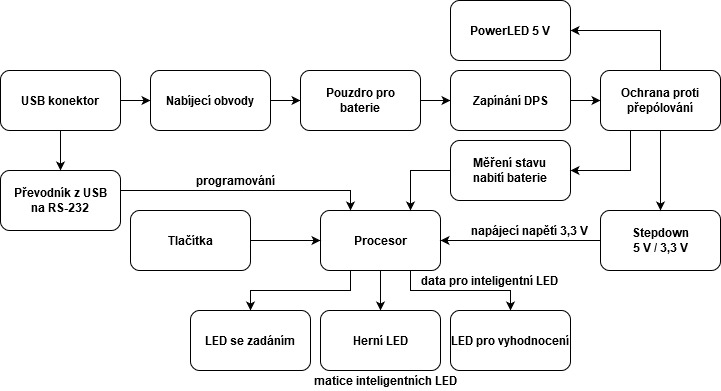
\includegraphics[scale=0.5]{obrazky/v0_blokove_schema.jpg}
    \end{center}
    \caption[Blokové schéma zapojení verze~0.0]{Blokové schéma zapojení verze~0.0.}
  \end{figure}

  \begin{figure}[!h]
    \begin{center}
      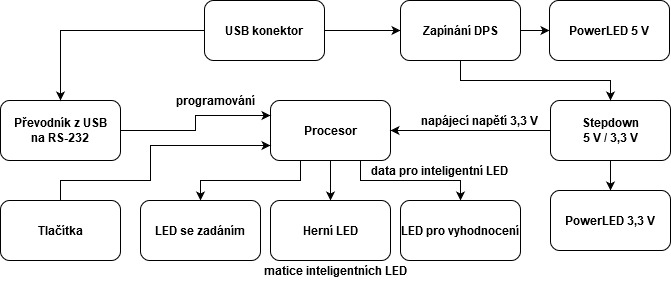
\includegraphics[scale=0.5]{obrazky/v1_blokove_schema.jpg}
    \end{center}
    \caption[Blokové schéma zapojení verze~1.0]{Blokové schéma zapojení verze~1.0.}
  \end{figure}

  Asi největším rozdílem mezi verzí~0~a~1 je způsob napájení. Verze~0 je napájena z~baterií a~verze~1 je napájena z~USB. Díky této změně 
  odpadly i~mnohé části obvodu. Díky absenci baterií bylo možné postrádat nabíjecí obvody, ochranu proti přepólování a~měření napětí 
  na bateriích.       

  \section{Napájení}
  \subsection{Verze~0.0}
  V~první verzi byly pro napájení použity baterie Li-Ion INR18650-29E od firmy Samsung. Tyto baterie mají jmenovité napětí 3,7~V, 
  při plném nabití až 4,2~V. Kapacita jedné baterie je 2850~mAh \cite{18650}. Byly použity 2~články baterií, které byly zapojeny paralelně. 
  Paralelním zapojením se celková kapacita zdvojnásobila.

  Baterie typu Li-Ion jsou náchylné na podvybití. Verze~0.0 proto obsahovala i měření napětí na bateriích. Pokud by došlo k~podvybití, mohla 
  by se bateriím zmenšovat kapacita, nebo by se mohly zničit. 

  Pro baterie bylo vybráno pouzdro na 2~články s~THT montáží do DPS \cite{18650_pouzdro}.

  Baterie byly připevněny a~zapájeny přímo do DPS, a~proto musel být integrován i~nabíjecí obvod. Nabíjení probíhalo přes konektor USB~Micro.

  Pro nabíjecí obvod byl zvolen čip TP4056. Tento obvod byl vybrán, protože je přímo určen pro nabíjení baterií typu Li-Ion. Existují 
  moduly pro nabíjení těchto baterií, které mají integrovaný tento čip \cite{Nabijeci_modul}. Tyto moduly jsou často používané, a~proto 
  bylo zapojení tohoto modulu převzato do této práce. 

  Vlastnosti čipu jsou přizpůsobeny bateriím Li-Ion. Nabíjení baterií probíhá do 4,2~V, což je maximální napětí na použitých 
  bateriích \cite{18650} \cite{TP4056_datasheet}. Díky tomu nemůže dojít ke zničení baterií nabíjením.

  \begin{figure}[!h]
    \begin{center}
      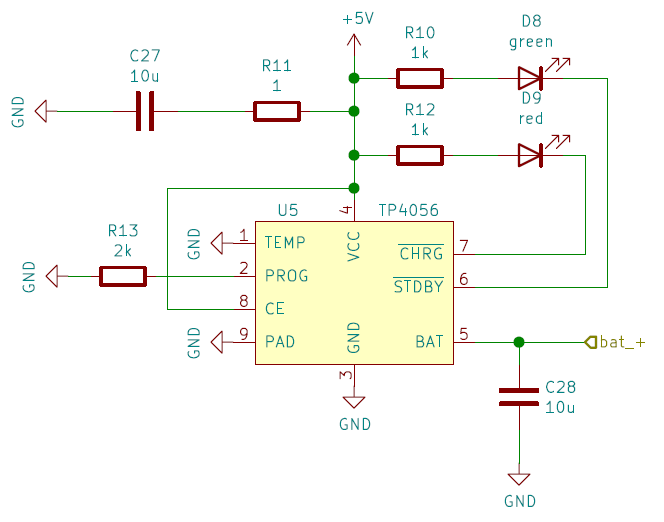
\includegraphics[scale=0.6]{obrazky/TP4056_schema.png}
    \end{center}
    \caption[Schéma zapojení čipu TP4056 \cite{TP4056_datasheet}]{Schéma zapojení čipu TP4056 \cite{TP4056_datasheet}.}
  \end{figure}

  Červená LED~D9 indikuje nabíjení baterií a  zelená LED~D8 svítí, pokud jsou baterie nabité \cite{TP4056_datasheet}. 
  Pokud nesvítí ani červená ani zelená LED, znamená to, že baterie jsou podvybité, baterie nejsou vloženy a~nebo je příliš vysoká, 
  nebo nízká jejich teplota \cite{TP4056_datasheet}.

  Rezistorem R13 se určuje nabíjecí proud baterií \cite{TP4056_datasheet}. Aby baterie nabíjením nebyly poškozovány, měl by být nabíjecí 
  proud maximálně 0,5~C (polovina kapacity baterie). Vybraná baterie má kapacitu 2850~mAh. Nabíjecí proud proto může být až 1425~mA. 
  Jelikož je pro tuto hru důležitější kapacita baterie, než doba nabíjení, byl zvolen nabíjecí proud pouze 0,5~A. Čím menším proudem 
  je baterie nabíjena, tím má delší životnost a~pomaleji ztrácí svoji kapacitu.

  \begin{table}[!h]
    \caption{Nastavení nabíjecího proudu rezitorem R13 \cite{TP4056_datasheet}.}
    \begin{center}
      \begin{tabular}{|c|c|}
          \hline
          R13 [k$\Omega$] & Nabíjecí proud [mA] \\
          \hline
          10      & 130 \\
          \hline
          5       & 250 \\
          \hline
          4       & 300 \\
          \hline
          3       & 400 \\
          \hline
          2       & 580 \\
          \hline
          1,66    & 690 \\
          \hline
          1,5     & 780 \\
          \hline
          1,33    & 900 \\
          \hline
          1,2     & 1000 \\
          \hline
      \end{tabular}  
    \end{center}
  \end{table}

  Byl zvolen rezistor o~hodnotě 2~k$\Omega$, kterým byl určen nabíjecí proud 580~mA. 

  \subsection{Verze~1.0}
  Ve verzi~1.0 byl změněn způsob napájení. Napájení v~této verzi neprobíhá přes baterie, ale pouze přes USB konektor, přes 
  který ve verzi~0.0 probíhalo pouze nabíjení baterií. 

  Výhody
  \begin{itemize}
    \item absence drahých baterií,
    \item absence nabíjecího obvodu,
    \item absence hlídání stavu nabití baterie,
    \item absence ochrany proti přepólování (USB konektor je uzpůsoben svým tvarem, aby uživatel nemohl napájení přepólovat.),
    \item napájení inteligentních LED napětím přímo z~USB (Inteligentní LED mají menší odběr proudu.).
  \end{itemize}

  Nevýhody
  \begin{itemize}
    \item předpokládá se, že uživatel vlastní powerbanku,
    \item výdrž závisí na kapacitě powerbanky. 
  \end{itemize}

  Byl zvolen konektor USB~Micro, protože se jedná o~nejrozšířenější USB konektor dnešní doby.

  \section{Vzhled DPS}
  %dopsat
  
  \section{Oživení prototypů}
  \subsection{Verze 0.0}
  DPS přijde z~výroby ve stavu, kdy jsou osazeny pouze SMD komponenty.

  \begin{figure}[!h]
    \begin{center}
      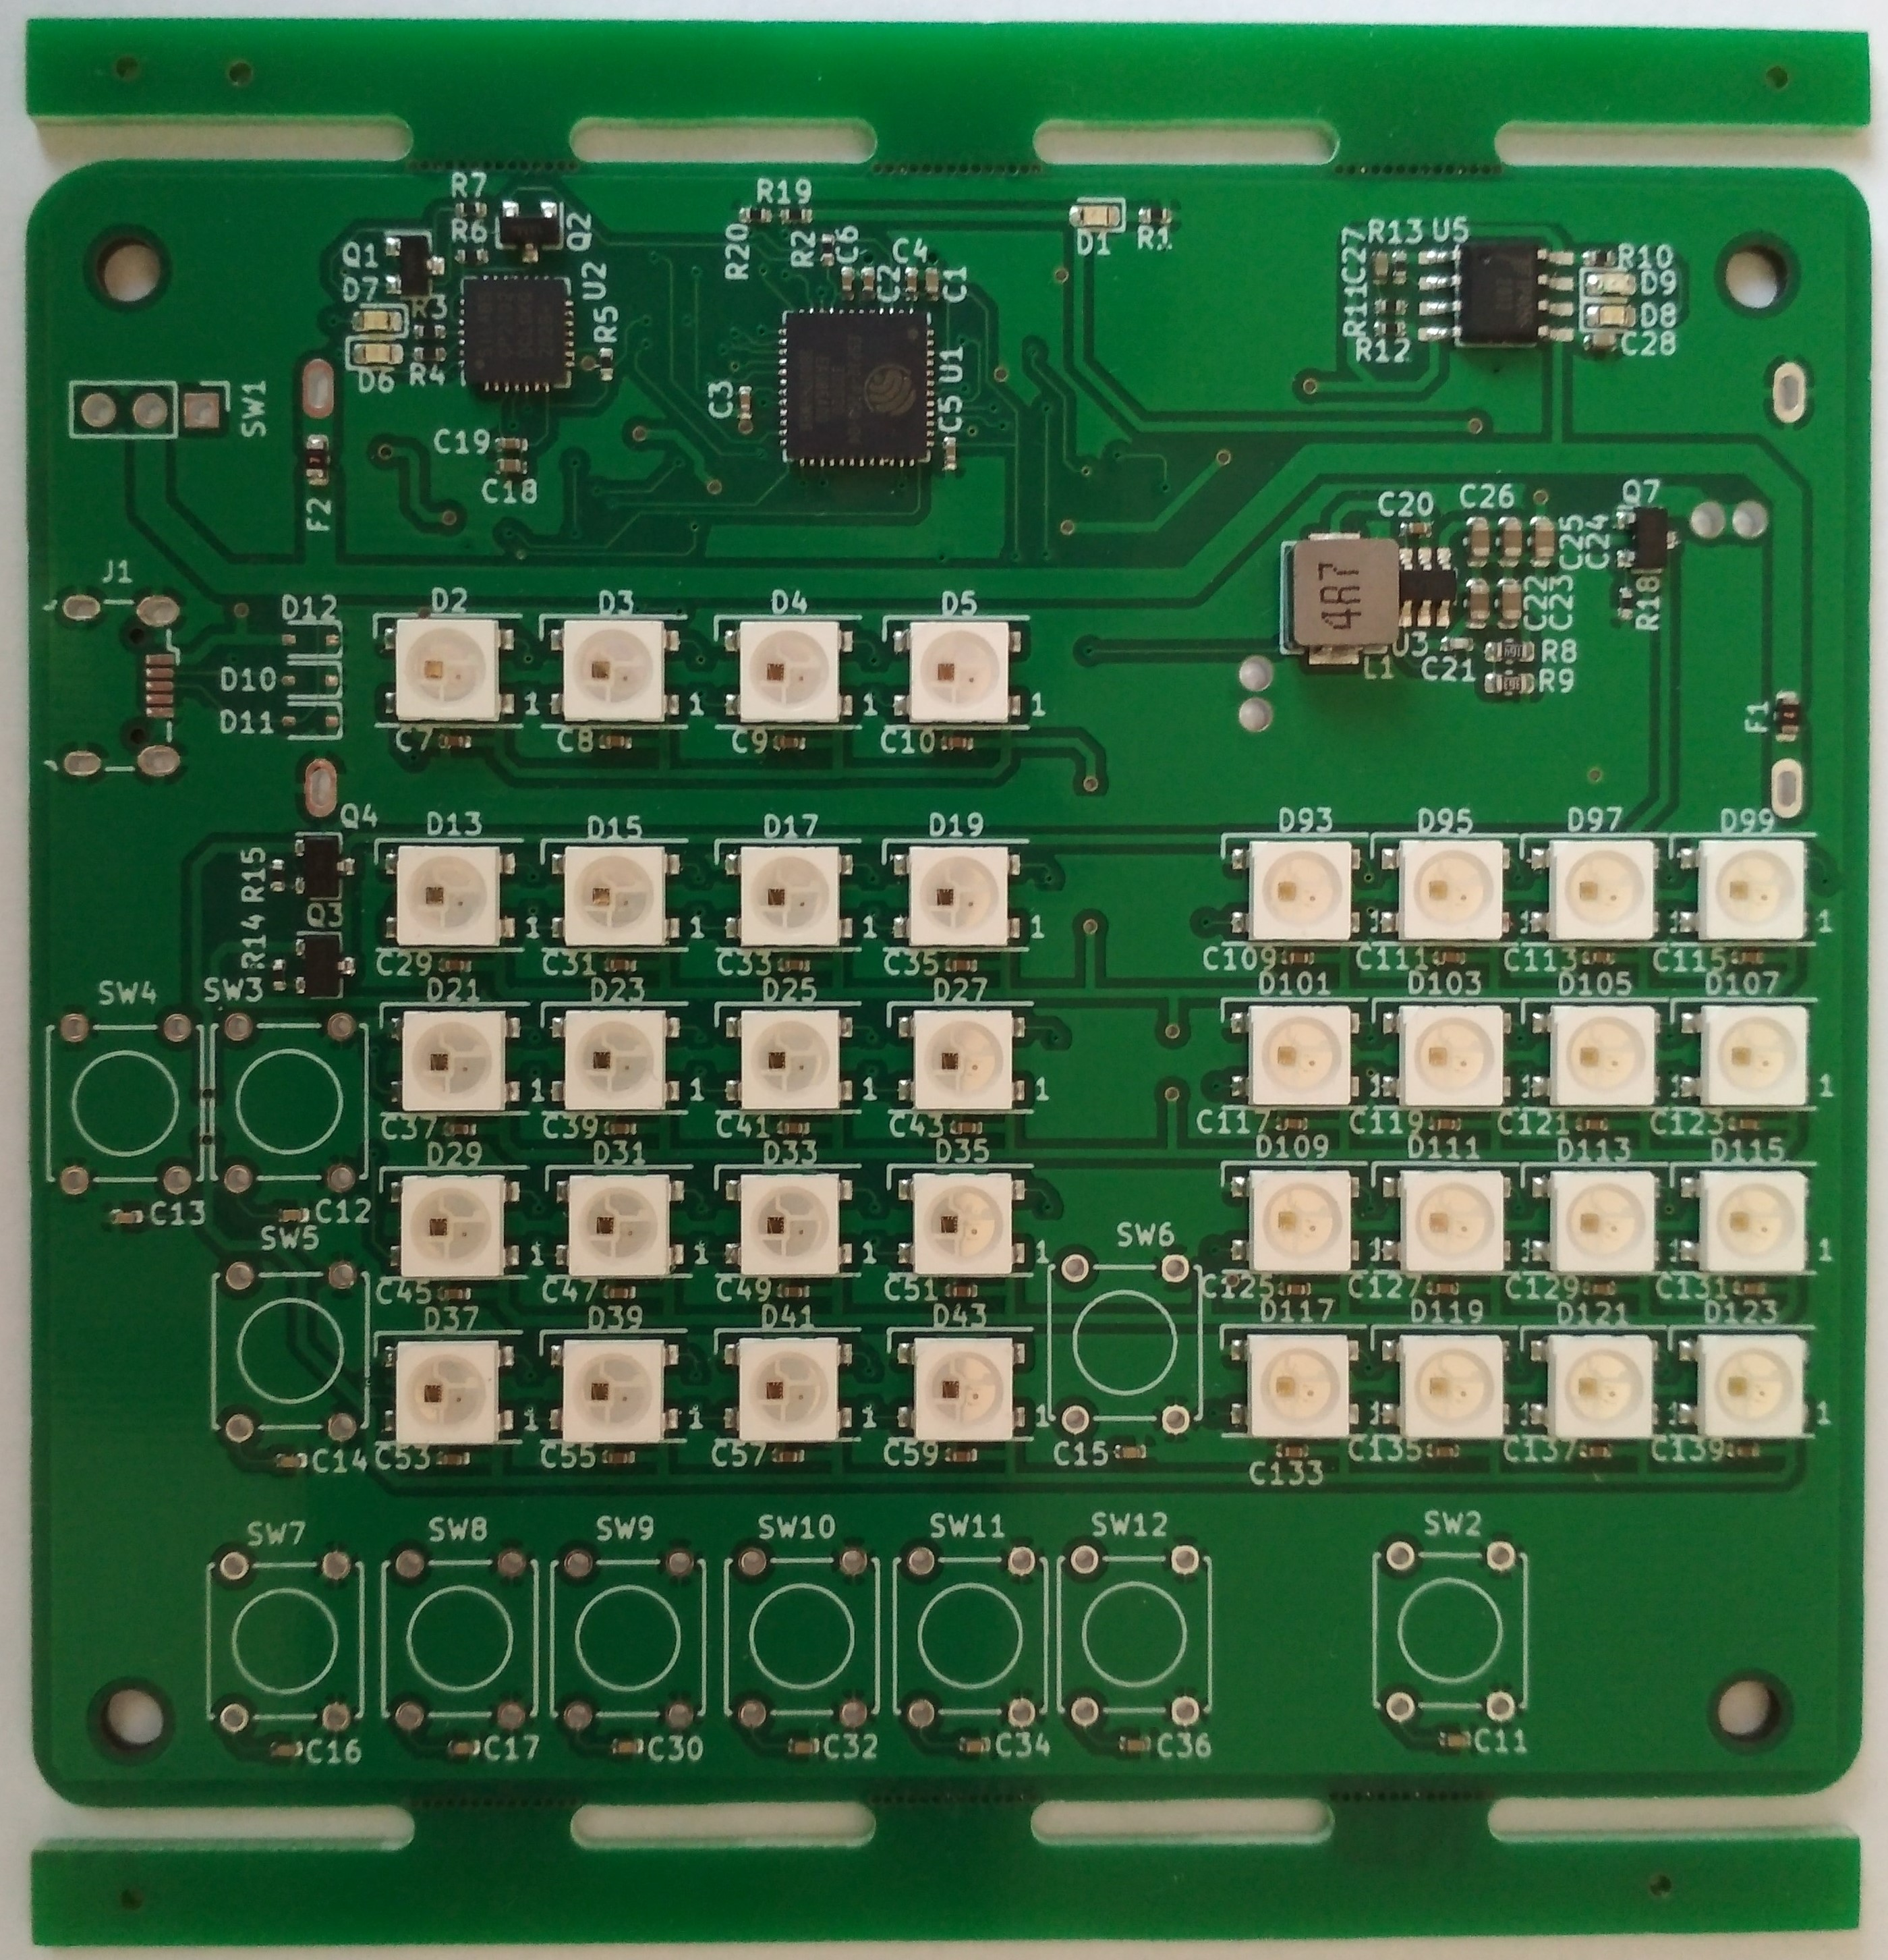
\includegraphics[scale=0.1]{obrazky/Verze0_vyroba_kolejnice.jpg}
    \end{center}
    \caption[Verze~0.0 z~výroby]{Verze~0.0 z~výroby.}
  \end{figure}

  Po dodání DPS z~výroby byly zapájeny THT komponenty (pouzdro na baterii, konektor USB micro, tlačítka a~vypínač). Na testovací verzi
  byl místo vypínače osazen konektor, na který je pro zapnutí DPS potřeba nasunout propojku. Po zapojení baterií
  18650 do pouzdra a~zapnutí vypínače se rozsvítí zelená LED~D1, která indikuje přítomnost napájecího napětí. 

  Po vložení baterií do pouzdra a~zapnutí DPS bylo pomocí multimetru zjištěno, že ochrana proti přepólování baterií nepropouští napětí 
  dále, i~když jsou baterie v~pouzdře umístěny správně. Bylo zjištěno, že pouzdro tranzistoru zajišťujícího ochranu proti přepólování 
  neodpovídá navrženému pouzdru tranzistoru. Všechny MOSFET tranzistory byly stejného typu, takže musely být všechny otočeny.
  
  Při zkoušce nabíjení bylo zjištěno, že červená LED indikující nabíjení baterií je přepólovaná. LED se povedla otočit a indikace nabíjení 
  baterií z~USB byla v~pořádku. 
  
  Při programování byl zjištěn problém s~komunikací po lince RS-232. Bylo zjištěno, že LED pro indikaci komunikace po lince RS-232 jsou 
  špatně zapojeny, a~proto byly odstraněny a~nahrazeny zkratem. Jejich zapojení této komunikaci bránilo. Bipolární tranzistory byly 
  taktéž osazeny ve špatném pouzdře a~neodpovídaly navrženým pouzdrům. 
  
  Při programování a~testování všech inteligentních LED WS2812C a~tlačítek bylo zjištěno, že jedno tlačítko bylo zapojeno na pin, který 
  nemá softwarově zapínatelný pullup rezistor. Tento rezistor byl dodatečně osazen.
  
  Po veškerých opravách byla DPS připravena na testování softwaru elektronické hry Logic.

  \begin{figure}[!h]
    \begin{center}
      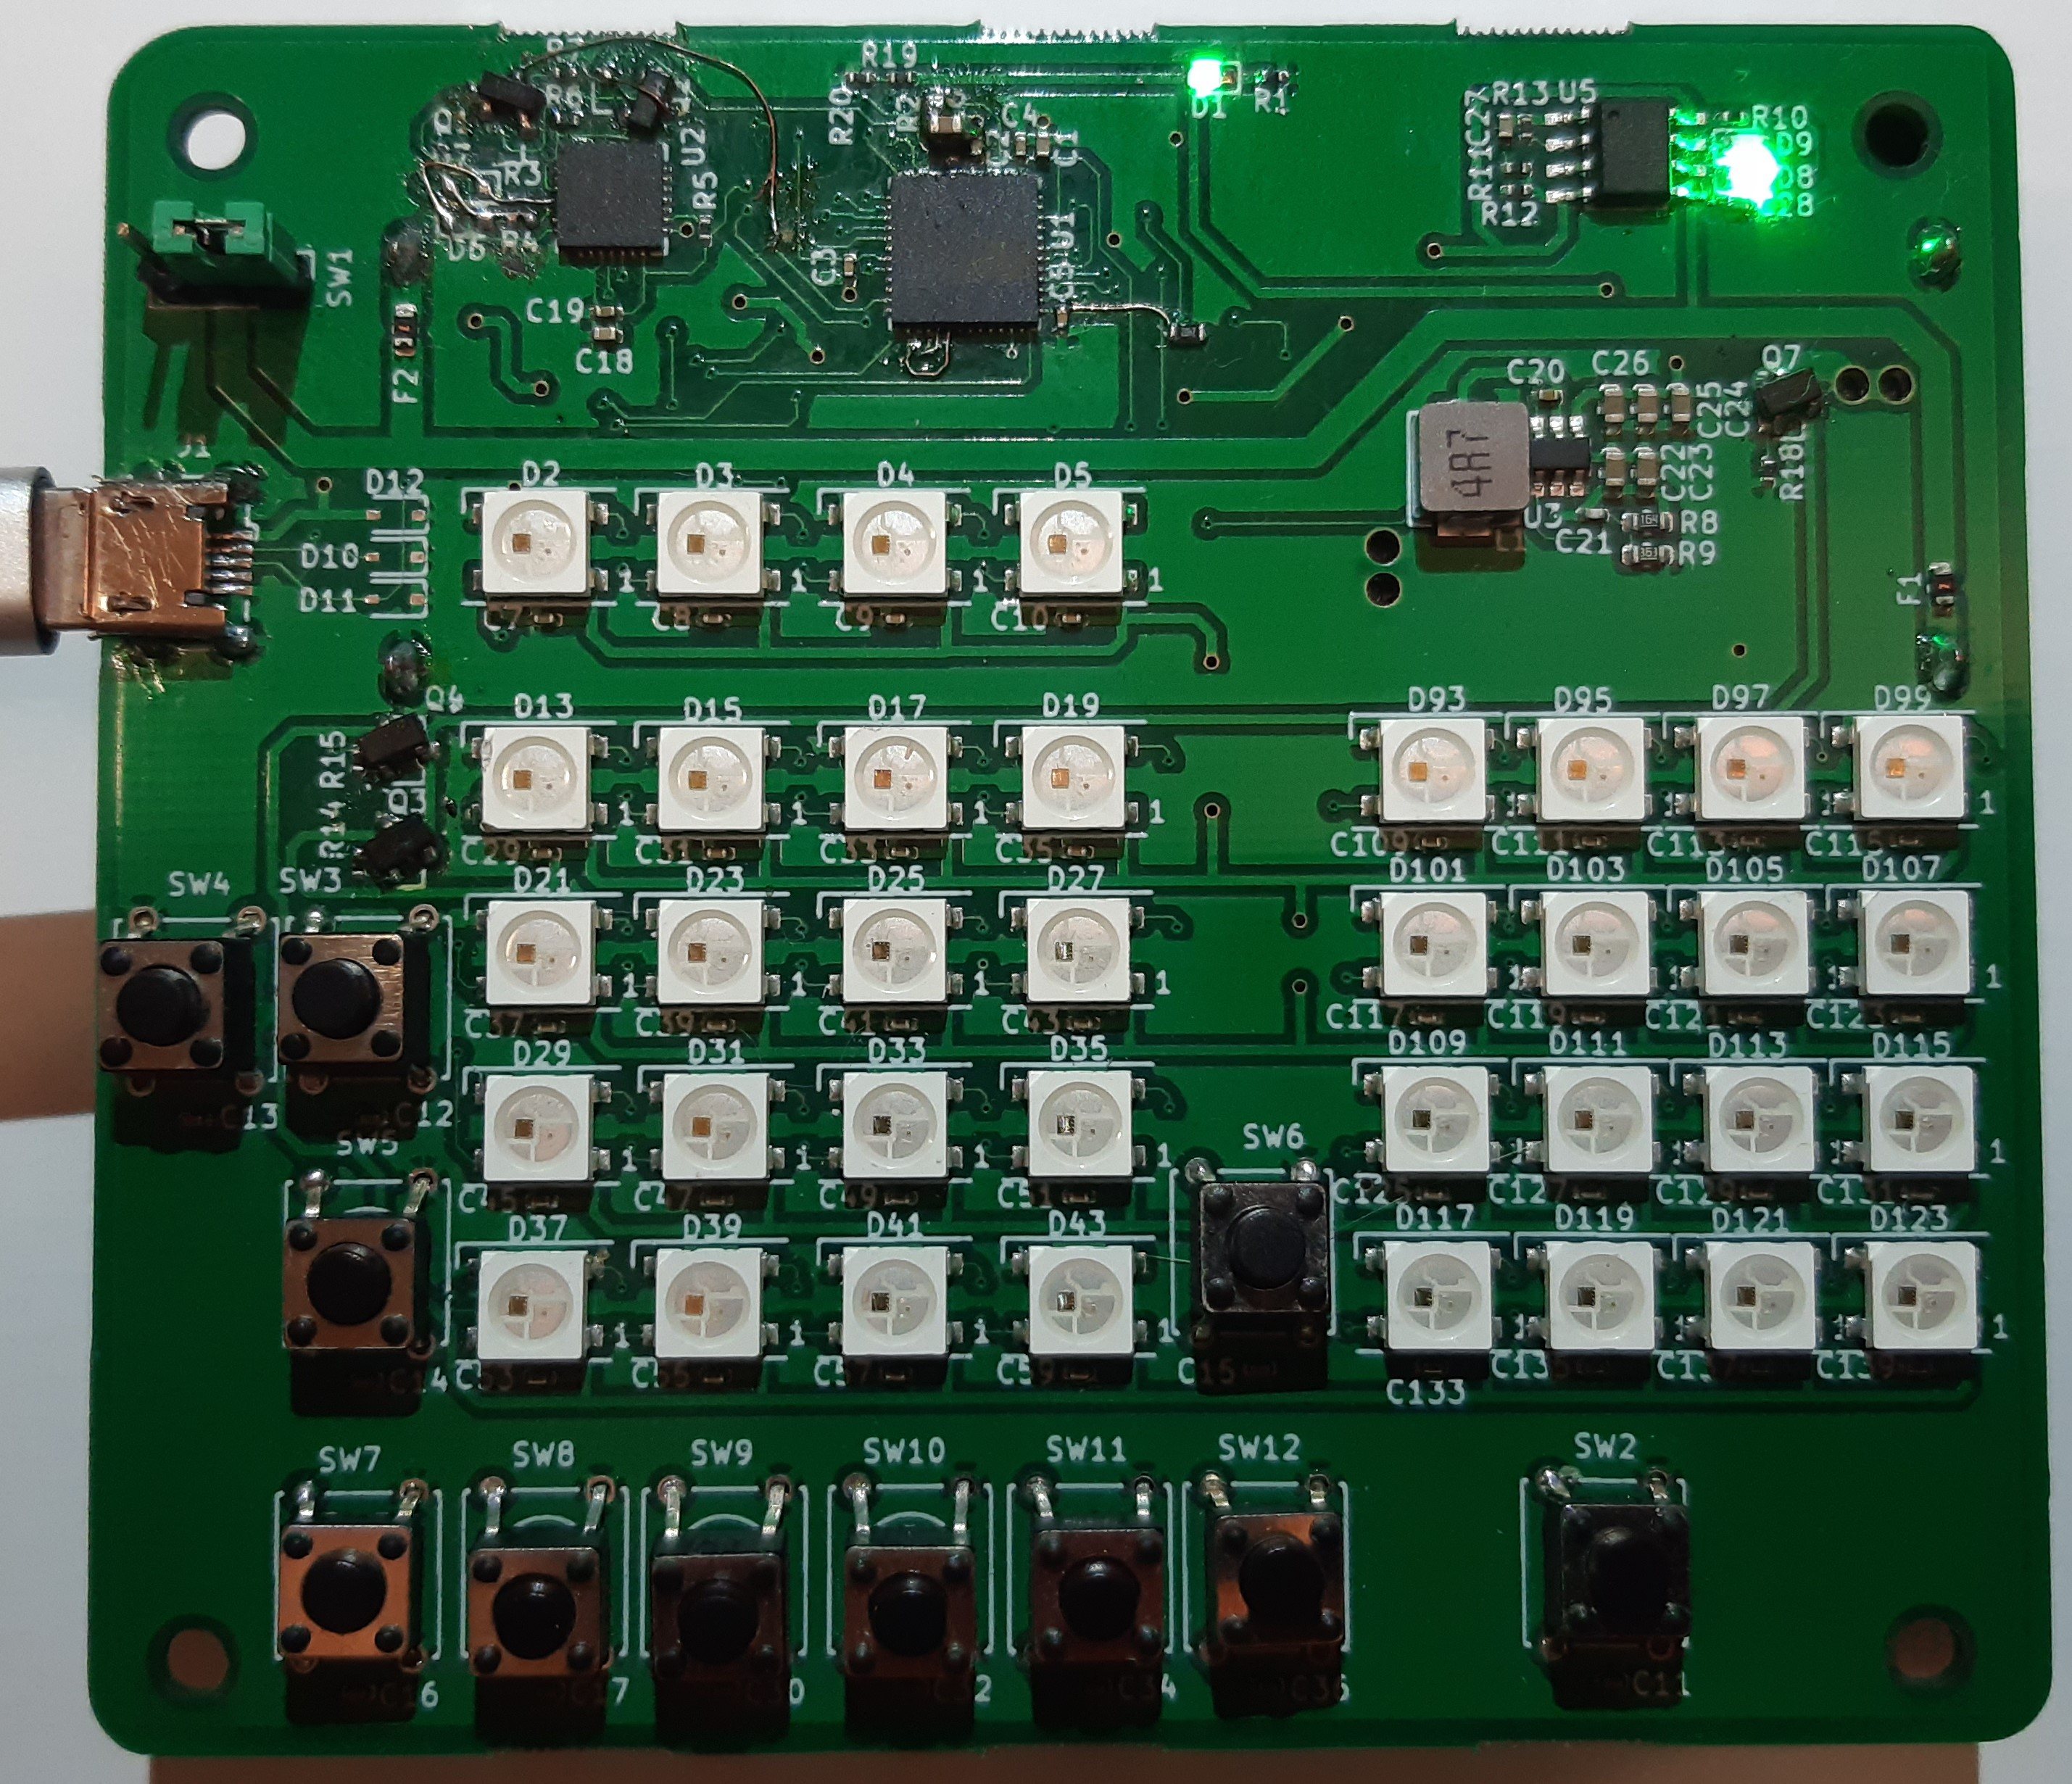
\includegraphics[scale=0.1]{obrazky/Verze0_zapnuto_nabito.jpg}
    \end{center}
    \caption[Oživená verze~0.0 s~opravami]{Oživená verze~0.0 s~opravami.}
  \end{figure}

  \subsection{Verze~1.0}
  DPS přijde z~výroby ve stavu, kdy jsou osazeny pouze SMD komponenty. 

  \begin{figure}[!h]
    \begin{center}
      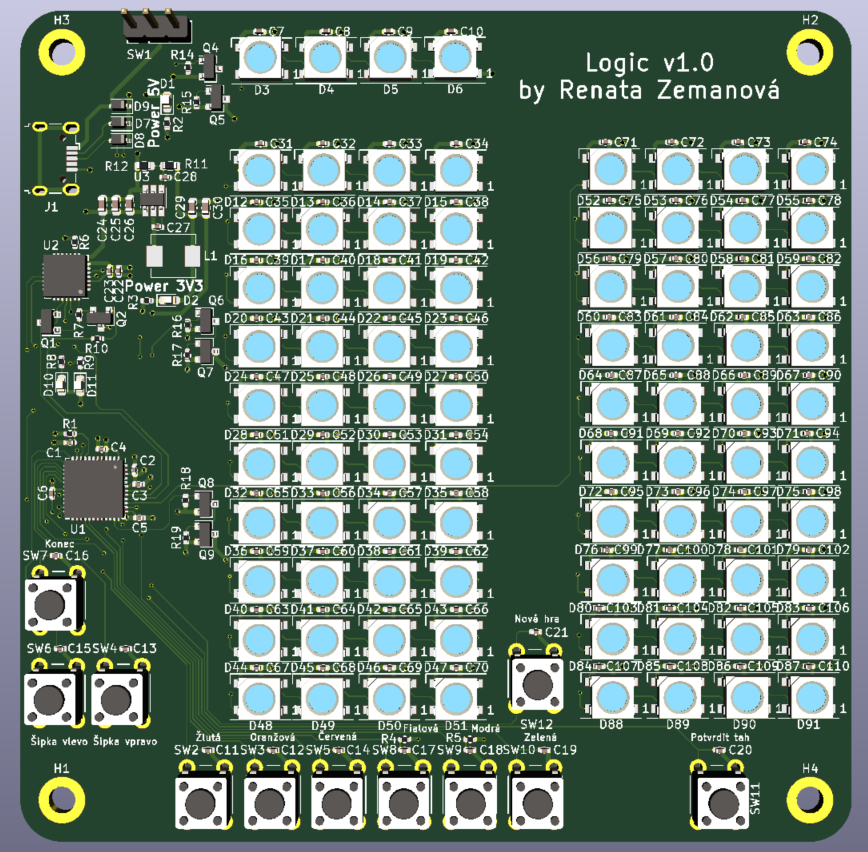
\includegraphics[scale=0.65]{obrazky/Verze1_3D_pohled.png}
    \end{center}
    \caption[3D~pohled verze~1.0 DPS]{3D~pohled verze~1.0 DPS.}
  \end{figure}

  Poté je nutné ručně osadit THT součástky, tj. vypínač, tlačítka a~konektor USB micro. Po připojení DPS přes USB konektor k~powerbance, 
  nebo do počítače, se rozsvítí LED~D1~a~D2, které indikují přítomnost napájecího napětí. LED~D2 zároveň značí, že zapojení měniče
  napětí je funkční.

  Tato firma v dnešní době 
  velmi rychle rozšiřuje svůj sortiment k osazení. Od výroby prototypů začala tato firma osazovat nejen SMD součástky, ale také THT.

  Všechny chyby z~předchozí verze byly odstraněny.

  

 
  




